\documentclass[11pt]{article}
\usepackage[top=1.00in, bottom=1.0in, left=1.1in, right=1.1in]{geometry}
\usepackage{Sweave}
\renewcommand{\baselinestretch}{1.1}
\usepackage{graphicx}
\usepackage{natbib}
\usepackage{amsmath}
\usepackage{gensymb}
\usepackage{parskip}
\usepackage{xcolor}
\usepackage[disable]{todonotes}
\usepackage{xr-hyper}
\usepackage[utf8]{inputenc}
\externaldocument{workingdraftsupp}

\def\labelitemi{--}
\parindent=0pt

\begin{document}

\renewcommand{\refname}{\CHead{}}

% See also: git/grants/crc2023/crc2023app/docs/crc_notes2023more.tex which has some reference notes

\title{Why longer seasons with climate change may \\ not increase tree growth} 
% Climate change highlights fundamental gaps in\\ plant growth $\times$ growing season length relationships  
% Do growing season length and growth relate? \\ And if not, why not? \\ And if we're not sure, why is that?
\author{Team Grephon}
\date{\today}
\maketitle



\begin{abstract} % 200-ish words
%CJC 15Dec - small edits around conciseness 
Recently a growing number of studies have challenged a fundamental assumption of most forecasts of future climate climate---that longer growing seasons lead to increased tree growth---which can partly offset carbon emissions. A suite of diverse hypotheses, from drought-related late season constraints to internal limits on plant growth, provide diverging explanations of why longer growing seasons do not always increase tree growth. Here, using a literature review spanning regional, continental and global scales, we find an almost even divide in how often increased growing seasons are linked to increased growth---with 58\% of all papers finding a positive relationship across over 56 species. We also found a fundamental disconnect between relevant fields---especially the two currently leading most research: dendrochronology and plant physiology. Major hypotheses are generally studied by one field with little interdisciplinary research, limiting any development---or testing---of a mechanistic framework for when longer seasons should lead to greater growth. Leveraging current research, combined with theory from evolutionary biology, community ecology and life history, we outline how progress towards a predictive framework is possible, but will require both new fundamental science, alongside new approaches within and across disciplines.  
\end{abstract}
% Ruben: We present a path towards building a mechanistic framework to predict the effect of longer seasons on tree growth. We suggest that lack of cross-disciplinary collaborations,and inconsistent terminology and testing approaches, are likely to explain why tree growth-phenology mechanisms remain poorly understood or outright untested. We discuss how easily accessible or already available data, currently untapped, has the potential to advance our understanding in this critical issue, and in turn greatly improve vegetation models.
% OLD: Here we highlight how progress could come from rising to the interdisciplinary challenge of this topic. Working across dendrochronology, ecology, life history, and physiology, we present a mechanistic framework for predicting when longer seasons should lead to greater growth.  While persistent biases in which disciplines study which mechanisms means much of the framework remains untested, we show that critical data---currently untapped---could rapidly advance our understanding, and in turn greatly improve vegetation models. % and highlight how poorly tested most mechanisms are.

\section*{Introduction} % 4,550 words currently 

The idea that longer growing seasons lead to increased plant growth is an intuitive tenet across multiple fields of biology, including physiology\todo{addcites}, dendrochronology \citep{frank2022dendrochronology} and ecosystem ecology. It is also a foundational assumption of most models of the future global carbon cycle \citep[e.g.][]{friedlingstein2022global, ito2020global}. Most models project that continued anthropogenic warming will be partly offset by increased carbon sequestration, primarily of temperate and boreal forests, as warming lengthens growing seasons\todo{addcites}, an assumption supported by a suite of ecosystem-scale studies \citep{chen1999effects,keenan2014net,finzi2020}. Yet recent work has called this assumption into question.

%CJC 15Dec - small edits 
A suite of recent studies have suggested longer growing seasons do not always lead to greater tree growth \citep{dow2022warm,green2022limits,silvestro2023longer}, with potentially large implications for future climate change. This research suggests that limitations on plant growth mean forests could be limited sinks with increased warming, despite longer growing seasons. Such findings challenge decades of research that find growth increases with longer seasons, from studies along natural elevational gradients\todo{addcites} to small-scale studies of cell growth in lab settings\todo{addcites} to studies of ecosystem fluxes with warming \citep{chen1999effects,keenan2014net,finzi2020}. Proposed mechanisms for the apparent disconnect are diverse (Fig. \ref{fig:hypotheses}), including previously unknown internal limits on plant growth \citep{zohner2023effect} and the complex effects of climate change itself, such as increased drought or temperatures too high for plant growth \citep{dow2022warm}, as well as differences simply due to the metric of growth \citep{green2022limits}.
% Studies that Green \& Keenan say no relationship:
	% Fatichi et al. 2014 (opinion)
	% Fatichi et al. 2019 (review)
	% JIang et al 2020 (FACE or sinilar) 

% Our approach spans multiple fields to unify foundational studies with recent research related to anthropogenic warming. Leveraging a systematic literature review, we examine in which methods, species and approaches extended seasons appear to lead to increased growth, and the current proposed hypotheses. 
%CJC 15Dec - small edits 
Here we review the connections between growing season length and plant growth across fields to identify the potential mechanisms that unite---and could disconnect---these processes. % Our approach spans multiple fields, from foundational to recent studies.  
Leveraging a systematic literature review, we examine which methods, species and approaches suggest that extended seasons appear to lead to increased growth, and the current proposed hypotheses. We find a pervasive disciplinary split between studies, which---we argue---limits our ability to identify the underlying processes and mechanisms. Further, we highlight critical insights from physiology, community ecology, evolutionary and life history theory that have been unexamined in recent work. With insights from these other fields and an interdisciplinary focus, research studying connections between growing season length and growth appear primed to develop a holistic theory of when, where and how climate change may increase tree growth---with implications both for forecasts of future climate change and for fundamental science.
 % JHRL(Nov2023): I know this would make the sentence long, but I want to say that we are primed to get the insights but only if we take the opportunities (lizzie adds: And make the first sentence much more exciting; maybe move up: we highlight critical insights from physiology, community ecology, evolutionary and life history theory that have been unexamined in recent work)

\section*{Evidence that longer seasons increase plant growth, or not}
%  (spanning 36 papers and 59 unique tests or studies; see Supp or Fig/Table)
%CJC 15Dec - attempt to clean up these first couple of sentences 
The idea that time limits growth is a fundamental principle of most biological fields. From the cellular to ecosystem levels, many biological processes are rate-limited in ways that tie back to time. Thus, the hypothesis that longer growing seasons should increase growth is intuitive---and pervasive. 

%CJC 15Dec - lots of "growth" happening. cleaning up a bit for conciseness 
The hypothesis that longer seasons yield more time for growth was by far the most common hypothesis for why longer seasons should increase growth across our review of growth $\times$ growing season length studies, with 19 of 59 total studies including it (Fig. \ref{fig:hypotheses} and see Supplement for review details). Foundational evidence for this relationship comes primarily from spatial clines across elevation and latitude, with growth decreasing alongside growing season length at higher elevations and latitudes (Fig. \ref{fig:gxelev}). Mechanistically, this hypotheses is supported by warming experiments that find that species which advance phenologically with warming also perform better \citep[with performance most often measured by growth,][]{Cleland:2012}. With climate change, ecosystem-scale studies have reported a similar positive relationship between growing season length and carbon fluxes across decades \citep{keenan2014net} or in years with warm, early springs \citep{chen1999effects}. These findings, however, have not been well supported by recent work that has focused often on inter-annual correlations with metrics of individual tree growth \citep{dow2022warm,silvestro2023longer}. This has led to debate about whether future carbon forecasts are overestimated and which metrics of growth \citep{green2022limits}, or growing season length \citep{korner2023four} are relevant.

Despite the recent eruption of this debate, we found little support for reports of a wholesale disconnect between growth and growing season length. Instead, research has generally found split support---across methods---for when longer seasons lead to increased growth. Papers spanning 25 years have variously found evidence for---or not---the relationship, with no clear trend by method, though a surprising number of papers never directly tested the relationship (Fig. \ref{fig:heatmaps}). Thus, the path to understanding these results is unlikely to emerge solely through improved metrics. 

Studies from the disciplines of dendrochronology (the study of tree rings and their dating) and physiology have readily offered mechanisms for the recent results that increased growth may not come with longer seasons. Hypotheses focus on both source (photosynthesis-limited, including $CO_2$ limitation) and sink limitations (Fig. \ref{fig:temperaturecomplex}). External climatic drivers that offset the positive growth effects of longer seasons are often reported in tree ring studies\todo{addcites} (and discussed in XX studies, see Fig. \ref{fig:hypotheses}), suggesting that higher temperatures paired with lower precipitation produce negative correlations with growth\todo{addcites}. In contrast, several other studies suggested fundamental internal constraints that prevent trees from responding to longer seasons, even without such external climatic constraints\todo{addcites} (see Fig. \ref{fig:hypotheses}). 

%JHRL Nov2023: the term 'other major possible mechanisms' is a bit vague - be more specific?
Yet we found that these hypotheses have been tested in radically different ways, never together, and ignore a suite of research on this topic---including other major possible mechanisms. Tree-ring studies have focused on external climatic drivers limiting growth in annual tree ring studies, while lab experimental and wood phenology (xylogenesis) studies focus on physiological constraints. Further, the inconsistency of results, with no clear pattern by method or even within species (Fig. \ref{fig:sppfinds}), suggests that understanding the relationship mechanistically will be critical to accurate predictions. As we outline below, a single mechanism is unlikely to explain all results, requiring a more unified framework, and tests of it, for progress. 
 
\section*{Controllers on growth $\times$ growing season length relationships}

% Here we examine the mechanisms that may limit or disrupt longer growing seasons leading to increased growth, integrating across the fields of dendrochronology, physiology, phylogenetics and ecology. 
A suite of mechanisms, representing both both external drivers---including climatic and biotic---and internal constraints, could prevent a universally positive growth $\times$ season length relationship. Currently, the lack of integration of several relevant fields and a tendency to focus on only select mechanisms within fields obscures this potential reality. Below we discuss findings across the fields of dendrochronology, physiology, phylogenetics and ecology to review the major mechanisms that may limit or disrupt the positive effects of longer growing seasons on growth, from individual (organismal) to community levels. 
% Currently, a the lack of integration of several relevant fields and a tendency to focus on only select mechanisms within fields obscures this reality. It also means we have little understanding of how mechanisms compare, or which may explain current findings.

\subsection*{External}

\paragraph{Temperature \& moisture} % Abiotic

Fundamentally, temperature limits many biological processes. Temperatures that are too cool (often considered to be below 5\degree C for temperate trees) and too warm \citep[an area of active research,][see also Fig. \ref{fig:temperaturecomplex}]{martinez2008hot,cabon2022cross} slow down biological processes and eventually can lead to tissue death \citep{larcher1980,kramer2012book}. Between the upper and lower limits biological processes underpinning growth generally accelerate such that warming can have a direct effect, effectively by accelerating biological time, up until the maximum rate for that particular process.

Anthropogenic warming will thus shift a number of biological processes at the same time that it accelerates spring phenology, but how big the shift is due to temperature will depend on the particular response curve and exactly where along that curve warming will push the process. At very cool temperatures, a small increase in warming may have limited effect, whereas warming that pushes plants beyond their optima, where many biological rates crash, could have large impacts. In between, warming would linearly increase rates. Plant growth is likely then to shift with extended growing seasons at the same time it shifts due to changing rates, with some papers suggesting longer seasons effectively only extend the very cool periods and thus have no discernible effect on growth\todo{addcites}, while others suggest observed increases in growth are due only to increased growth rates (not longer seasons). A number of tree ring studies %CJC 15Dec - add in num of tree ring studies x temperatures from our lit review here or from Fig S1??
suggest an offset of increased growth (due to longer seasons) from high summer temperatures \citep{gantois2022new,dow2022warm}, though which temperatures are too high is not generally known, and it seems likely current temperatures are below most plausible optima \citep{schaber2002evaluation}, unless other factors, such as drought, decrease that optima (Fig. \ref{fig:hypotheses}f). 

% JHRL Nov2023 suggests adding the below:
% Of course, warming has complex effects on climate-relevant environmental factors, altering not just growing season length, but potentially also drought, frost, etc. Some of these factors may have opposite impacts of growth, offsetting positive effects of growing season length on growth. Adding even greater complexity, these plant-relevant climatic factors are differentially limiting depending on macro climate, which means that it can be difficult to generalize about growing season length impacts on growth, without considering other warming related factors 
Positive effects of longer seasons on growth could also be offset by moisture deficits. If warming reduces soil moisture through either reduced precipitation or higher evaporation it could slow growth dramatically. A suite of tree ring studies confirm this, finding correlations with precipitation\todo{addcites} or other metrics related to plant access to water\todo{addcites}. The actual relationship between temperature, moisture and tree growth is more complex, as studies finding strong correlations between vapor pressure deficit and growth attest\todo{addcites}. 
%CJC 15Dec - again possibly add in numbers here looking at tree ring x precip studies??
% Temperature response curves assume sufficient moisture, with growth rapidly slowly ....

\paragraph{Species interactions} % Biotic

External factors related to species interactions---including herbivory, disease and competition---can also limit growth, and may themselves be responsive to an extended growing season. For example, herbivory can have large impacts on forests, leading to declines in satellite measures of greenness often associated with signals of plant senescence\todo{addcites}. Plant pathogens are also known to respond to warming, and limit productivity. These biotic drivers of growth have rarely been mentioned in studies examining growing season length (we found no mention of them in our literature review, Fig. \ref{fig:hypotheses}e), but could be increasingly limiting growth in some areas as extended growing seasons allow for additional generation cycles in many pest species \citep{mitton2012mountain,lange2006thresholds}.
% Kavya Nov2023: maybe we can connect this bit more to the hypothesis figure by mentioning the increased risk with an earlier growing season as an example of how herbivory/pests might impact growth

\subsubsection*{Internal}

\paragraph{Universal limits \& triggers} 
Fundamental limits on plant processes through biophysical realities may limit the extent to which growth can increase in response to a greater growing season length \citep[e.g., allometry, chemical reaction limits, and genetic architecture that may limit what trait combinations are possible,][]{ackerly2000evolution}. Additionally, long-term exposure to early- and late-season risks (e.g. frost) and growth constraints (e.g. low water availability) may have selected for a limited growth response to extended growing seasons. Regardless, when and how growth is initiated and ceases is clearly under genetic and / or developmental control, and thus, plants internal programming could limit growth responses to longer growing seasons. Some recent studies suggest a novel role for the summer solstice \citep{zohner2023effect} in setting a universal developmental switch between when warming temperatures hasten or delay leaf senescence (thus influencing growth season length and growth). However, these studies contradict decades of work showing species-level differences in how and when species grow.  % This is hypothesized to be universal, somewhat contradicting decades of work showing local adaptation by populations, and species-level differences in `determinism' in growth x growing season length relationships. 

\paragraph{Species-specific limits}
The underlying genetic and developmental drivers of growth varies by species, as evolution generally drives selection for different optima and different strategies (Fig. \ref{fig:hypotheses}c). For example, leaf strategies vary strongly between evergreen and deciduous species, but also within each group---where variation in `determinism' defines a suite of differences in the levels and timing of investment and leaf growth. Determinate species build most of their leaf material the season before and flush most leaf buds all at once at the start of season, while indeterminate species more continually produce new buds and flush them. Such differences can clearly influence the extent to which the growth of different species is influenced by increases in growing season length, even under identical conditions.%% CJC 15Dec - do we have any studies that look at the difference btw deciduous or coniferous? Or maybe we could count up the studies that look at "taxonomic variation" in the "what.endo" column?

% Ideas of determinism, often used in forest science, intersect with ecological theories of different plant strategies along which species---within communities and on biogeographical scales---assemble. 
Whether and how strongly increased growing seasons result in increased growth can potentially also be understood by considering differences amongst species in their life history strategies. Leaf, wood, fruit and other plant traits show trade-offs along a acquisitive to conservative axis, where some species can grow rapidly and more flexibly take advantage of resources, but are less defended against herbivores and compete poorly at low resource levels, whereas other species compete well at low resource levels, but at the expense of growing slower and conservatively \citep[][]{Grime:1977sw,diaz2016}. These ideas would predict indeterminate acquisitive species, such as poplar, to be far more likely to grow more with longer seasons, while conservative species, such as beech, may not.   %CJC 15Dec maybe this is the 1 source limitation study?
% Also say ring vs diffuse porous?
% Such strategies may also make predictions for reproductive investment, which---along with species-level differences---is almost wholly ignored in the current debate on the relationship between growth and growing season length.

Species differences in growing season $\times$ growth relationships, regardless of their direction, do not always reflect optimal strategies today. Imprints of past selection, also drive species-level differences, producing phylogenetic patterns that both limit how well species are adapted to current conditions and especially constrain their responses to rapidly changing conditions \citep{Ackerly:2009ly,phenophylo}. The legacy of historical evolutionary pressures---including different external drivers---is not easily erased.  Thus, many species show evidence of previous selection, seen when evolutionary relationships (usually represented through phylogeny) predict plant responses and lead to clade-level similarities. Most studies testing for such historical effects on plant responses find them \citep[e.g.,][]{phenophylo}, and even more physiological syntheses find results suggestive of strong phylogenetic relationships \citep[though they are more rarely formally tested, e.g.,][]{way2010differential}. 

\paragraph{Population- \& individual-level limits}
Below the species-level, populations and individuals also vary in their growth and its responses to growing season length (Fig. \ref{fig:hypotheses}d), similarly reflecting differences in genetic and developmental controls. For example, populations often vary predictably in their end-of-season phenology, with more poleward populations tending to stop height growth (budset) earlier using locally adapted photoperiod cues \citep{soolanayakanahally2013timing,aitken2016}. This means longer seasons---when the end of the season is as defined by budset---are generally driven by spring phenology, which appears far more flexible, and has advanced more rapidly than fall events \citep{aitken2016}. Within populations, individual trees may also vary in how early or late they are for both spring and fall events. This can be driven by maturity and a shifting investment to growth, survival and / or reproduction. Saplings, for which growth and survival are paramount, tend to both grow more rapidly and have longer seasons relative to adult trees. The response of adult trees may then vary depending on their investment in reproduction. 

% Kavya Nov2023: this matches with the <U+201C>shifting allocation<U+201D> in the hypothesis figure. However, the way the text is written right now is more like this vegetative-reprodictive trade-off leads to species/population differences instead of being a fundamental source of not increased growth with longer GS
Trade-offs between vegetative and reproductive investments are a paradigm of life history theory and may also produce important growth response differences across years within individuals (as well as between species). Years of high reproductive output can reduce growth \citep{thomas2011bookchptr,hacket2016tree}. For species that mast---producing abundant cones or fruits in only some years---high reproduction years could especially impact measures of wood growth. Many hypotheses suggest higher summer temperatures trigger masting in the following year \citep{hacket2016tree,hacket2016consistent}; if true, then reduced growth in years following warm summers may not indicate temperatures too high for growth, as often suggested \citep[e.g.,][]{gantois2022new,dow2022warm}, but instead shifting investment in reproduction.

\section*{An interdisciplinary framework for growth $\times$ growing season length relationships}
% "Crossdisciplinary: viewing one discipline from the perspective of another. Multidisciplinary: people from different disciplines working together, each drawing on their disciplinary knowledge. Interdisciplinary: integrating knowledge and methods from different disciplines, using a real synthesis of approaches."
 
 % Building a mechanistic framework of when and where... 
 % These levels of complexity across diverse external and internal drivers make a suite of testable predictions.
Predicting when and where longer seasons lead to increased growth may seem overwhelming given the diversity of potential drivers, but together they offer a set of testable hypotheses that could rapidly advance progress---if tackled with a more organized interdisciplinary approach. Most fields studying growth $\times$ growing season length relationships consider a limited set of metrics and a small subset of possible drivers (see Figs. \ref{fig:heatmaps}, \ref{fig:heatmapssupp}). Beyond failing to test a suite of highly relevant mechanisms, the lack of interdisciplinary study means we lack coherent tests that compare multiple mechanisms. Taken together, the current landscape of research suggests we may be testing hypotheses for how plants shift with climate change that we never previously understood well in fundamental biology. 
% Most fields studying this include a limited set of metrics and consider only a small subset of potential factors, with entire suites of hypotheses missing from the literature (see Fig. XX). 

% Beyond failing to test a suite of highly relevant mechanisms, the lack of interdisciplinary study means we lack coherent tests that compare multiple mechanisms. Dendrochronology considers almost exclusively external climatic drivers, while physiological tests of constraints do not usually predict for which species, when and where constraints will be most important. Taken together, the current landscape of research suggests we may be testing a hypothesis for shifts with climate change that we never previously understood well in fundamental biology. 

Below we outline a path towards building a better mechanistic framework for predicting when the longer growing seasons caused by anthropogenic climate change will increase plant growth. This path requires building fundamental biological knowledge in a suite of areas across physiology, dendrochronology, life history, ecology and evolutionary biology. These suggestions thus apply to understanding this relationship at the individual (organismal) level, though they make predictions at larger (e.g., ecosystem) scales, and are highly applicable to ecosystems dominated by one species \citep[e.g.,][]{chen1999effects}. % These suggestions apply to those wanting to specifically address hypotheses about the relationship between growing season length, phenology and growth at the individual (organism) level

\subsubsection*{Standardized measurements} % Box?

Tackling the diverse drivers and their underlying hypotheses (Fig. \ref{fig:hypotheses}) for growth $\times$ growing season length relationships requires a common language and set of metrics for growing season length \citep{korner2023four}, growth (see Box), and the potential drivers. We found 14 different metrics of start and 16 metrics of end of season (25 metrics of growing season length), and 21 different metrics of growth across 59 studies---highlighting just part of the problem. Definitions and metrics for external and internal drivers were myriad, %CJC 15Dec - I think we could again add numbers for external and internal divers, clarifying these were after systematically assigning studies into groups
with many papers reporting dozens of tests of different aspects of climate over different temporal windows. This is understandable, given the complexity of environmental variables and our limited understanding of how they trigger phenology and growth, but also slows progress. A common framework where researchers measure and report common explanatory and response variables (see Supplement) would accelerate research by easing communication between fields and providing a path to comparable quantitative estimates. This should also include expected statistical tests, as we found a number of papers failed to directly test for growth $\times$ growing season length relationships (Fig. \ref{fig:heatmaps}). % A first fundamental need for any framework is comparable quantitative estimates---which we currently lack. 


\subsubsection*{Bridging the internal-external drivers divide}

% Careful interdisciplinary is critical, but will benefit from shifts within disciplines. 
Standardized measurements will not yield fully comparable estimates---especially on the relative impacts of external and internal drivers---without larger shifts within fields. Major fields studying this relationship---dendrochronology, phenology research and physiology---all need to broaden in specific ways to overlap with one another to facilitate interdisciplinary work. At the same time, all fields have missed certain major hypotheses they could test (Fig. \ref{fig:hypotheses}), highlighting the need to integrate perspectives from other disciplines with relevant theory and methods. 
% JHRL Nov2023: maybe also genomics and developmental biology

\paragraph{Quantify species/population/individual variation} 

% While tackling these challenges for multiple species alone can seem daunting, allowing for and studying differences between species may remove much of the noise in current studies. ... % Both fields yield expectations of which species should differ the most. 
%CJC 15Dec - this paragraph seems potentially redundant with portions of the \paragraph{Species-specific limits} above. I will help iron out later with fresh eyes! 
A robust interdisciplinary approach to understanding growth $\times$ growing season length will need to integrate disciplines that focus on variation at the species-level and below. To date, a handful of studies have mentioned species differences (see Fig. \ref{fig:hypotheses}) but almost none have made or tested predictions on how species differ based on existing theory. 

Life history theory, community ecology and evolutionary history predict---and find---relevant patterns of species-level variation. Species with acquisitive versus conservative traits, and which differ in their reproductive strategies (i.e., masting or not, fruit size and number) provide an axis of important variation that could be used to identify focal species for further study and to test predictions. Acquisitive species with consistent investment in fruit would show stronger shifts in growth with changing growing season length---assuming no other factors become limiting. Given the potential role of evolutionary history, selecting for these varying strategies within a clade, or---if not feasible---correcting for phylogenetic distance would more robustly test how strategies influence the growth $\times$ growing season length relationship. Given an increasing number of studies across more species, a careful synthesis of studies across species could further test for the role of evolutionary history. 

Explicitly including differences between species may explain some of the variation in current studies, and would allow tests of the scale of species versus population, individual, and within-individual variation. Community ecology and life history theory clearly predict that species are unlikely to share a common growth $\times$ growing season length relationship, but less research addresses how the relationship should shift across populations within species. \emph{In situ} elevation work suggests no genetic differences \citep{king2013tree}, while common garden studies across latitudes suggest phenological variation across populations can limit growth responses to extended growing seasons \citep{soolanayakanahally2013timing}. Current growth responses to anthropogenic climate change mostly operate one level further below these---at the intra-annual (within-individual) level. 

% Getting a handle on these levels of variation is important for as we need to understand the scale of it versus other levels of variation, and compared to other drivers of variation. Current studies of how growing season length influences growth have worked at a variety of scales corresponding with some of these levels, though most fields rarely mention or study this variation. The focus of physiology means they rarely consider variation beyond individuals. In dendrochronology, previous work across space likely compared populations, while recent studies have focused on inter-annual variation within individuals. Partitioning this variation requires studies that sample carefully at each level, then statistically separate out variation. 

Understanding the scale of variation across all these levels could both help to refine theory and provide a benchmark when comparing the effect sizes of other drivers of variation. While multiple papers report a lack of relationship between growth and growing season length, we have no fundamental understanding of what the effect size of this relationship should be, and thus no way to know if we have good power in current studies to detect it. Estimates of how growth shifts with elevation likely include responses from both plasticity (within-individual variation) and local adaptation (population-level variation) and thus could be an upper bound on our expectations, yet elevational trends to date appear relatively weak and noisy (Fig. \ref{fig:gxelev})---suggesting this is only part of our missing mechanistic understanding. 

\paragraph{Extending disciplinary focus} 

Each major field studying growth $\times$ growing season length (dendrochronology, phenology research and physiology) has its own historical aims, and thus its own biases towards certain species, methods and metrics. Dendrochronology's original focus on using tree growth to estimate climate has led to certain assumptions and methods  that likely obscure the complexity of how growth shifts with growing season length. Fundamentally, the field relies on an assumed relationship that, within individual and populations of trees, growth (measured by annual ring width) is greater when growing conditions are better \citep[e.g.,]{cook2013methods}.  Dendrochronologists traditional aim to magnify the climate signal has led to standard approaches, including sampling biases (e.g., to `climate-sensitive' individual trees) and statistical detrending (of tree ring chronologies), that may obscure patterns where the signal of effects of growing season length and biotic drivers (see below) may be most apparent \citep[such as rapid growth phases,][]{manzanedo2019towards}.  %Fundamentally, the field has long assumed growth decreases with shorter growing seasons \citep[e.g.,][]{bruening2017} over space, such as higher elevations and latitudes.%AKE: I have not read bruening but a skim of it suggests that it is not a tree ring paper- rather a treeline paper. do we still want to cite it here? I removed it but I can look for another one that is tree ring focused...
Unfortunately, these approaches mean dendrochronology studies are also fundamentally washing out much of what physiological studies focus on, limiting opportunities for interdisciplinary overlap. % Bridging this gap would be aided by physiological studies reporting metrics similar to ring width, alongside their more common measurements of shoot elongation, height and biomass. 

Opportunities for overlap between dendrochronology and phenology research are potentially higher that for dendrochronology and physiology, but sampling biases in both fields limit current opportunities. Dendrochronology's aim for prioritizing climatic response has led to a strong focus on conifers (gymnosperms), creating a major split from most studies of leaf phenology, which focus almost entirely on deciduous species, which are mainly angiosperms (see Fig. \ref{fig:hypotheses}). Phenology research has also been overly focused on spring events (e.g., budburst, leafout), with limited data on fall events and thus limited data to calculate growing season length. This focus on spring events may have been justified decades ago, when most shifts from anthropogenic warming occurred in the spring, but less justified as increasing research suggests important complexity in fall shifts \citep{gill2015,zohner2023effect} and a need to scale up phenological research to understand tree growth.

% Biotic/spp diversity for all ... 
All fields have lacked a focus on the ecology of growth $\times$ growing season length, generally ignoring impacts of certain external drivers, the complexity of life-history, and species differences. Dendrochronology often uses frost events or insect outbreaks as markers of particular years, but rarely integrates them into patterns of growth. A shift to reporting and estimating effects of frost events, biotic disturbances, and reproduction status of trees (including mast years) could provide new estimates of the effects of these drivers. Physiological studies tend to avoid such complexities through controlled environments and a focus on juvenile plant stages, but scaling up between life stages will be critical for useful models of growth, and to bridge to dendrochronology. % Both fields have also tended to ignore competition. Mechanistic physiology studies rarely measure or include competition and, given dendrochronology's focus on climatic signal through growth, the field similarly tries to avoid the study or impact of plant competition, even though it is foundational to forest dynamics.

\paragraph{Extending temporal focus: Zooming in and out}% Lags \& allocation

Bridging across disciplines will require bridging across timescales, a consistent and thorny issue for research on trees. We found most physiological studies of growth $\times$ growing season length relationships studied 1-2 years of dynamics, usually of juvenile trees, while tree ring studies are focused on synthesizing across decades or longer of adult tree growth. Perhaps because of this dichotomy, tree ring studies often study lag effects\todo{addcites}, while they are rarely mentioned in physiological studies. Given the complexity of carbon storage in trees \citep{finzi2020,thompson2023no,anderson2022drives}, and how investment can shift across years\todo{addcites}, studies should more consistently acknowledge and test for lag effects. % Now below: Integrating more research from ecology and field global change experiments could help. Large scale experiments on heat (e.g., SPRUCE), moisture via drought or irrigation (e.g., DroughtNet, Phynwald) and other factors (e.g., $CO_2$ in FACE) have increasingly been used to test ecological `memory' and could help scale up from smaller and shorter-time scale physiological studies.

% All fields would benefit from a deeper understanding of the physiological and/or developmental connections between growing season length and growth. Much work has focused on measures of growth and phenology without a clear mechanistic link. Similarly, many current suggestions of constraints lack any physiological mechanism. Physiological studies that follow carbohydrate and cell division versus expansion dynamics could yield insights. This is particularly important if want to include constraints in our projections, as extrapolating is especially dangerous when the underlying mechanistic model is wrong
All fields could benefit from tackling the challenge of understanding the physiological connections between growing season length and growth, and even the genetic and developmental underpinnings of these connections. To date, much work has focused on measures of growth and phenology without a clear mechanistic understanding of what triggers growth and the cessation of growth, and how these triggers and responses have evolved. This includes current suggestions of constraints that lack any physiological mechanism,
 %CJC 15 Dec - reference Fig S1 here - only 3 studies looked at external or internal factors by phenology.
 but progress in this area is could be particularly important for making projections, as extrapolating can be dangerous when the underlying mechanistic model is wrong. Physiological studies that follow carbohydrate and cell division versus expansion dynamics could yield insights, as could additional work on xylogenesis---especially if done with a focus both to extrapolate to long-term tree ring studies and/or in physiological experiments. Expanding beyond the current disciplines focused on this topic could also be informative. For example, a clearer understanding of which environmental stimuli trigger leaf expansion, senescence, and woody growth, the underlying developmental processes that are triggered, and their evolution, could contribute towards a clearer understanding of growth constraints.


\section*{Urgent opportunities}

% JHRL Nov2023: I think we want to differentiate this section from the previous. in the last, we provide somewhat general no brainer suggestions for any person doing this kind of study. Here, we suggest several specific approaches to take that should lead to very interesting insights. Maybe we need to describe these by the questions answersed, or be specific that these represent examples of the kind of interdisciplinary work we feel is needed? Not sure, but think these two sections need to be better distinguished.

\paragraph{Existing data and networks}

Expanding the focus of disciplines to help build an interdisciplinary framework for growth $\times$ growing season length relationships will take time, but some hypotheses may be tractably tested by taking advantage of existing data sets and ongoing experiments. We mention three such opportunities here. 

First, both dendrochronology and phenology research have large freely-available repositories of data, with the International Tree Ring Database (ITRDB) and the Pan European Phenology project (PEP725) being two of the largest. While each dataset reflects the biases previously mentioned, they also provide a major spatially and temporally diverse dataset to compare how external climatic drivers, species and population explain growth $\times$ growing season length relationships. Depending on the data overlap, these datasets may also allow us to identify  where longer growing seasons will increase growth and for which types of species. Based on existing theory, we expect longer growing seasons will increase growth for species with regular reproduction \citep[no masting, see also new masting database in][]{hacket2022mastree+}, an acquisitive strategy, from clades that are historically (on an evolutionary timescale) plastic, in locations that are warm---but not too warm---and moist.% Further, earlier growth should not drive increased frost damage, herbivory, or disease. Go test it, preferably in some mid-latitude, temperate forest for a species not too close to the edge of its range.

A second opportunity comes from existing common garden studies, from which more robust tests of population and individual variation could come. Given that many common garden studies have some data on phenology\todo{addcites} and are designed to tease out population versus inter-annual variation, collecting tree ring data from them seems a rapid way to estimate variation across these two levels. Repeating such measurements for multiple common gardens would also allow for an exploration of species level variation. Common gardens not collecting regular phenology, or annual growth data, could start. Given how old some common gardens are, research may also be able to examine impacts of biotic and abiotic disturbances or effects of climatic variation. 
% Common gardens not collecting regular phenology, or annual growth data, could start. 
% Common garden studies are designed to tease out population versus inter-annual variation, but the variation across these levels in growth $\times$ growing season length relationships is rarely studied. 

Finally, taking advantage of existing ecological and field global change experiments could help test lag effects, and bridge from physiological to dendrochronology scales. Large scale experiments on heat \citep[e.g., SPRUCE,][]{hanson2017attaining}, moisture via drought or irrigation \citep[e.g., DroughtNet, Phynwald][]{smith2016drought} and other factors (e.g., $CO_2$ in FACE) have increasingly been used to test ecological `memory' \citep[e.g., ][]{flinker2021promise, schweiger2022transgenerational} and could help scale up from smaller and shorter-time scale physiological studies, potentially to ecosystem-level dynamics such as carbon cycling \citep{ding2021plant, jensen2019simulated}. Building on available data and infrastructure could also bridge this gap, for example, adding dendrometers to locations with phenological sampling and vice versa. Such efforts may be especially valuable in sites across elevational and latitudinal gradients (e.g., PSP, Feeley elevation network, Coweeta). These sites in turn could be priority locations for xylogenesis and focused physiological studies. 

\paragraph{Next experiments}

Disentangling the effects of major drivers on growth $\times$ growing season length relationships will also require new experiments, across multiple levels. Teasing out the effects of warmer temperatures versus longer seasons can only be robustly done with experiments, and seems a paramount need, especially if done across multiple species spanning diverse strategies. Similarly, experiments to compare impacts of extended seasons (via early growth or delayed senescence), and differentiating between external abiotic (e.g., heat waves, droughts) and biotic (e.g., pests, competition) drivers could provide comparable estimates and test lag effects, when sampled multiple years after the manipulations (as opposed to immediately at the end of the treatment season). While these are most easily done for juvenile trees, they could also be done on adult trees, given the infrastructure investment. % Similarly, experiments to compare impacts of external biotic and abiotic drivers are critical---if carefully designed they would also provide insights on potential constraints.  

Efforts to design and launch such large-scale experiments should start now. A long-term experiment on adult trees that manipulates temperature, precipitation and growing season length, would test a suite of drivers at the relevant lifestage. Combined with careful measurements of carbon allocation, including to reproductive output, and tissue lost to frost and biotic drivers, such an experiment could rapidly compare a suite of drivers. With species carefully chosen to maximize divergent strategies and the potential for genomic and related studies (e.g., \emph{Populus, Quercus}), the experiment could also become a resource for studies of underlying mechanisms for constraints. At a larger spatial scale, distributed experiments to measure growth and phenology (ideally wood and vegetative) of multiple provenances of multiple species across sites could estimate variation---and potential constraints---that operate at different organizing levels. 

\emph{Conclusions:}
Anthropogenic climate change has often been described as an unfortunate, unnatural, accidental, and unreplicated experiment. It has highlighted important biology we don't know well, requiring us to rediscover dusty old fundamentals, and also expose their limits---and thus our limits of understanding. Understanding when, how and why longer seasons lead to increased tree growth requires an interdisciplinary reckoning with how temperature, growth and a suite of external and internal drivers affect plant growth. The task may seem large, but bridging across theory and data from dendrochronology, phenology research, physiology, evolutionary and life-history theory could rapidly advance fundamental biology in ways that translate directly to improved models of future forest dynamics, and the suite of species and services that depend on them. % And that includes carbon sequestration---which, we really need now! 

\emph{Acknowledgements:} N. Pederson for discussion, B. Wuu for extracting growth $\times$ elevation data. 

\iffalse

i. Hypotheses for why GSL x growth is not found are not equally tested across fields: Constraint issues in provenance but not tree ring etc.\\
ii. Our premise is that some hypotheses for what is going may be tractably already answered by combining data across fields/methods\\
iii. And, you could go far by cross-field tweaking of what each field is doing

Most global models of future warming assume increased anthropogenic carbon will be offset by increased carbon sequestration in forests as growing seasons lengthen.

The proposed mechanisms for this, however, are highly diverse---and most studies measure different aspects of growth across widely varying spatial and temporal scales. 

A positive link between longer growing seasons and increased carbon sequestration 

A suite of recent studies have called into question this fundamental assumption .... failed to find a link between longer seasons and increased tree growth

This assumption appeared well supported by several large-scale studies of ecosystem fluxes 
\fi


\newpage
\section{Box. ``Growth", measured how, exactly?}
Tree growth can be measured in a variety of ways. Our literature review found that most studies quantified growth by measuring radial growth (e.g., through increment cores or dendrometers, $n=$28), but a number also looked at metrics related to C assimilation (e.g. net ecosystem productivity or gross primary productivity, $n=$20), while a smaller number examined biomass, height, or number of stems ($n=$9), or root:shoot ratio ($n=$1). Some studies used modeled estimates of photosynthesis 
(e.g., \citet{smith2014implications} relied on daily photosynthesis estimates derived from the LPJ-GUESS photosynthesis model, while \citet{chen2000approaches} estimated photosynthese using the Integrated Terrestrial Ecosystem C-budget model, InTEC). Others measured photosynthesis at the leaf level, through flux towers, or used greenness metrics (NDVI). 

Growth measurements vary across disciplines and study types, posing a further challenge to an interdisciplinary approach to understanding how growing season length relates to growth. Greenhouse or growth chamber studies and provenance trials were more likely to measure height or biomass, whereas larger scale syntheses and remote-sensed studies are more likely to use metrics of carbon assimilation. 

Aligning across the range and scale of growth metrics will be critical for an integrated understanding of growth-growing season length relationships and implications under continued climate change.  There is decoupling among some metrics of growth. For example, vegetation photosynthesis may be poorly correlated with tree radial growth, and this relationship can vary seasonally \citep{cabon2022cross}. Further, tree radial growth is not a perfect indicator of whole tree growth, since plants allocate carbon to their roots, leaves, reproductive structures, and stores in addition to aboveground biomass. Relationships among different metrics of growth are not simple, so selecting relevant ones and aligning across the most widely used ones will be necessary, though not easy: the relationship  between photosynthesis, radial growth, and carbon uptake has large implications for future carbon sequestration and it remains widely debated \citep{green2022limits}. Further, there is a need to understand how to scale up across these varying metrics- from leaf and individual level to populations, communities, and ecosystems- while incorporating the variation that exists within and across levels.


\newpage
\section{Figures}


\clearpage
\begin{figure}[h!]
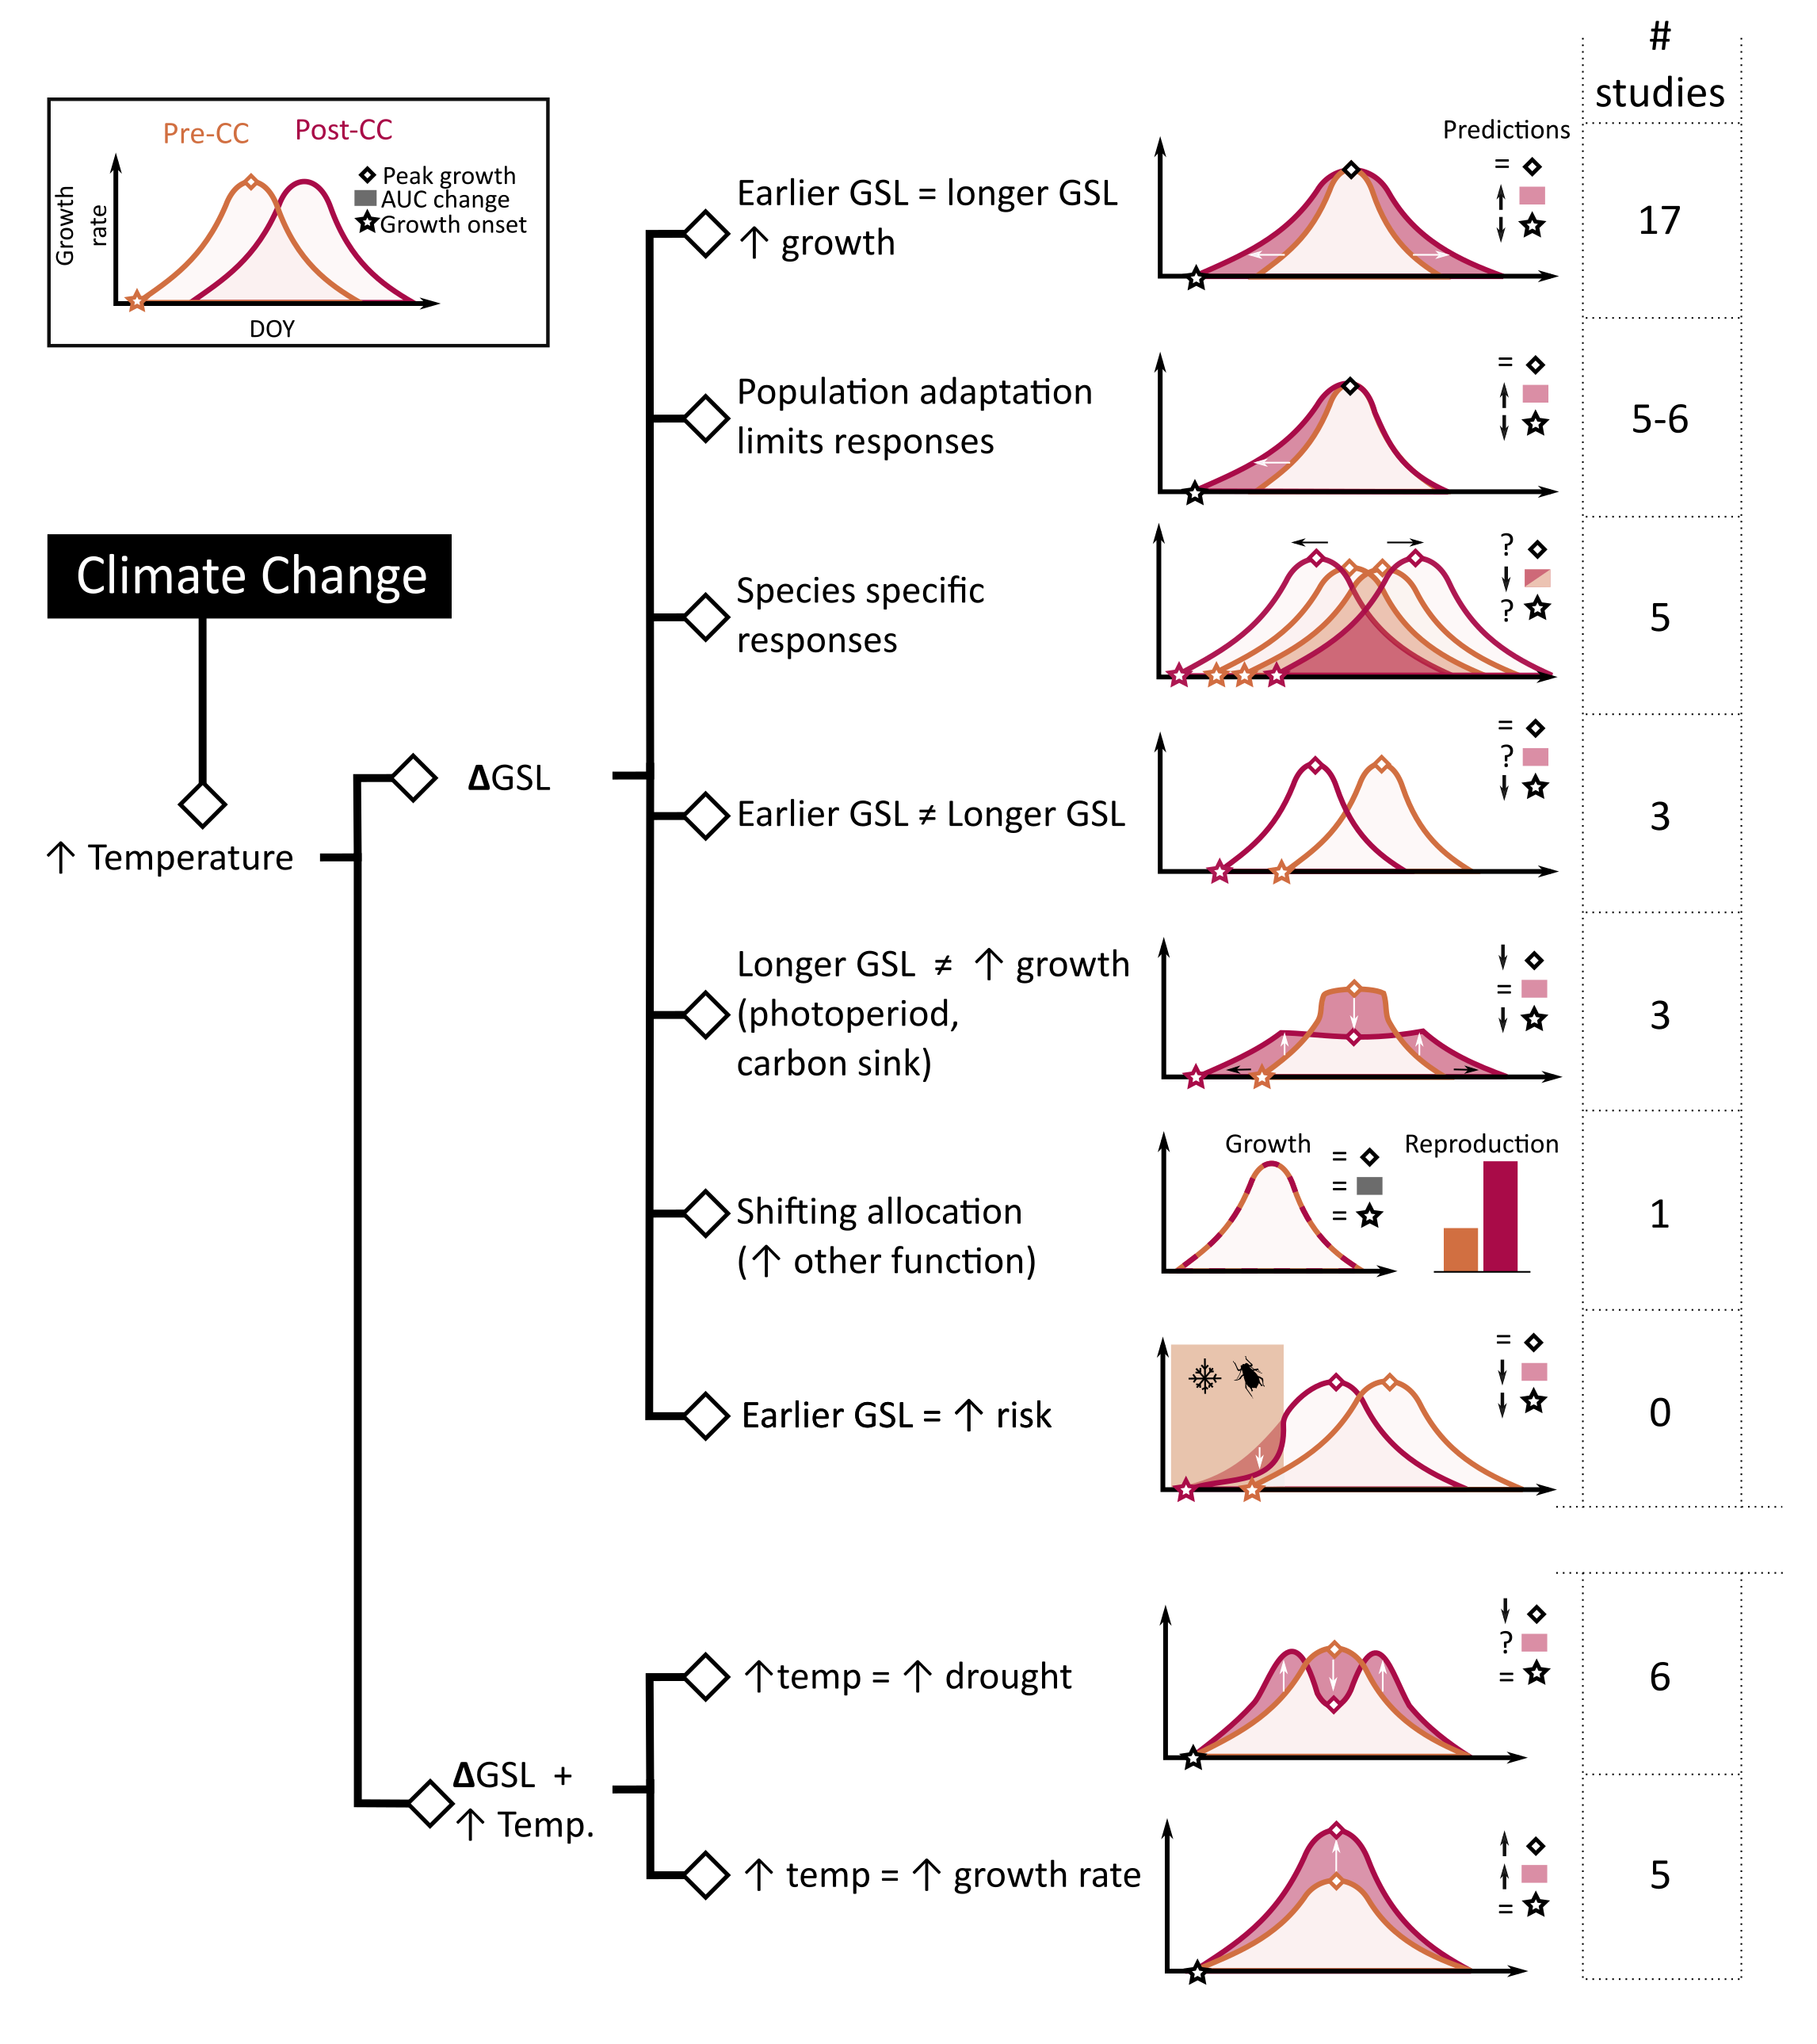
\includegraphics[width=1\textwidth]{..//figures/hypothesesconceptfig.png}
\caption{Pathways through which climate change could alter growing season length and growth.}
\label{fig:hypotheses}
\end{figure}

\begin{figure}[h!]
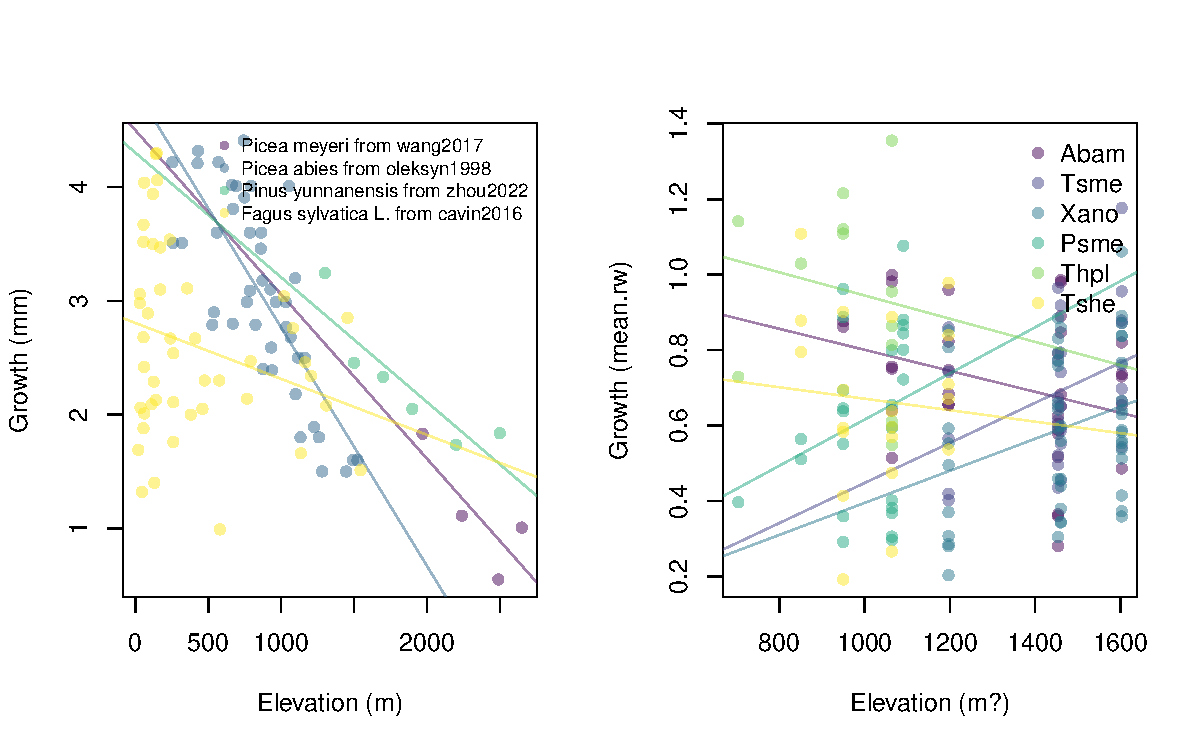
\includegraphics[width=1\textwidth]{..//analyses/growthxelevationetc/figures/growthxelev2part.pdf}
\caption{Growth $\times$ elevation studies (from the literature, left) and results from Mount Tahoma/Rainier (right).}
\label{fig:gxelev}
\end{figure}

\clearpage
\begin{figure}[h!]
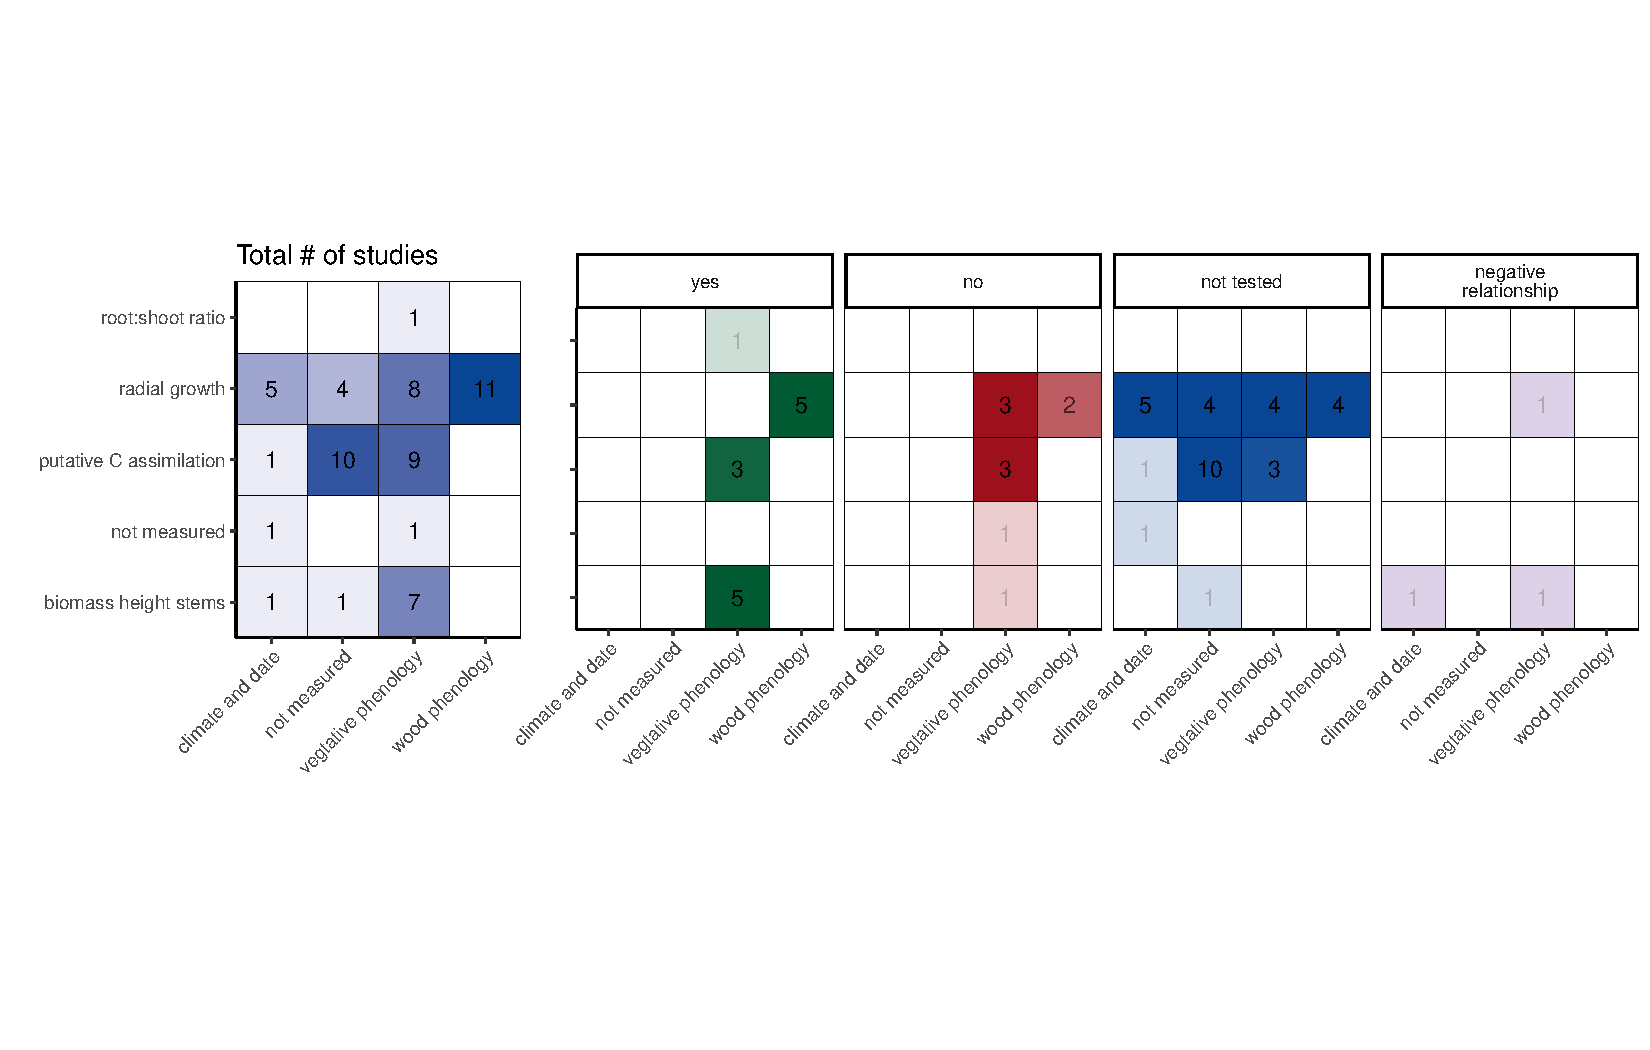
\includegraphics[width=1\textwidth]{..//figures/heatmaps/combinedheatmap_gslxgrowth_simple.pdf}
\caption{A review of the literature on growth $\times$ growing season length relationships spanned a diversity of methods, but there was no coherency in which methods did or did not find a positive relationship.}
\label{fig:heatmaps}
\end{figure}

\clearpage
\begin{figure}[h!]
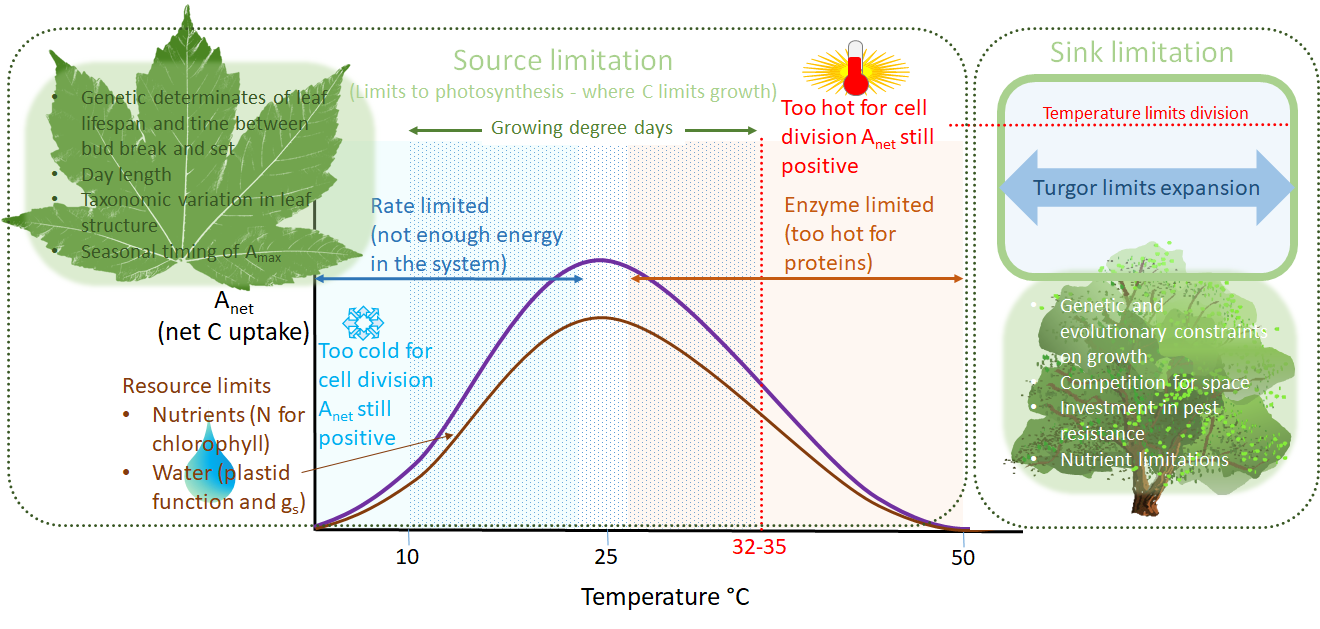
\includegraphics[width=1\textwidth]{..//figures/grephonfig.png}
\caption{Less simplified version of how temperature works, including lots of limits at high and low temperatures (we need to update to make more asymmetric and to have the language match the language in the paper more ... or we need to add a box to this figure to explain all the terms).}
\label{fig:temperaturecomplex}
\end{figure}

\clearpage
\begin{figure}[h!]
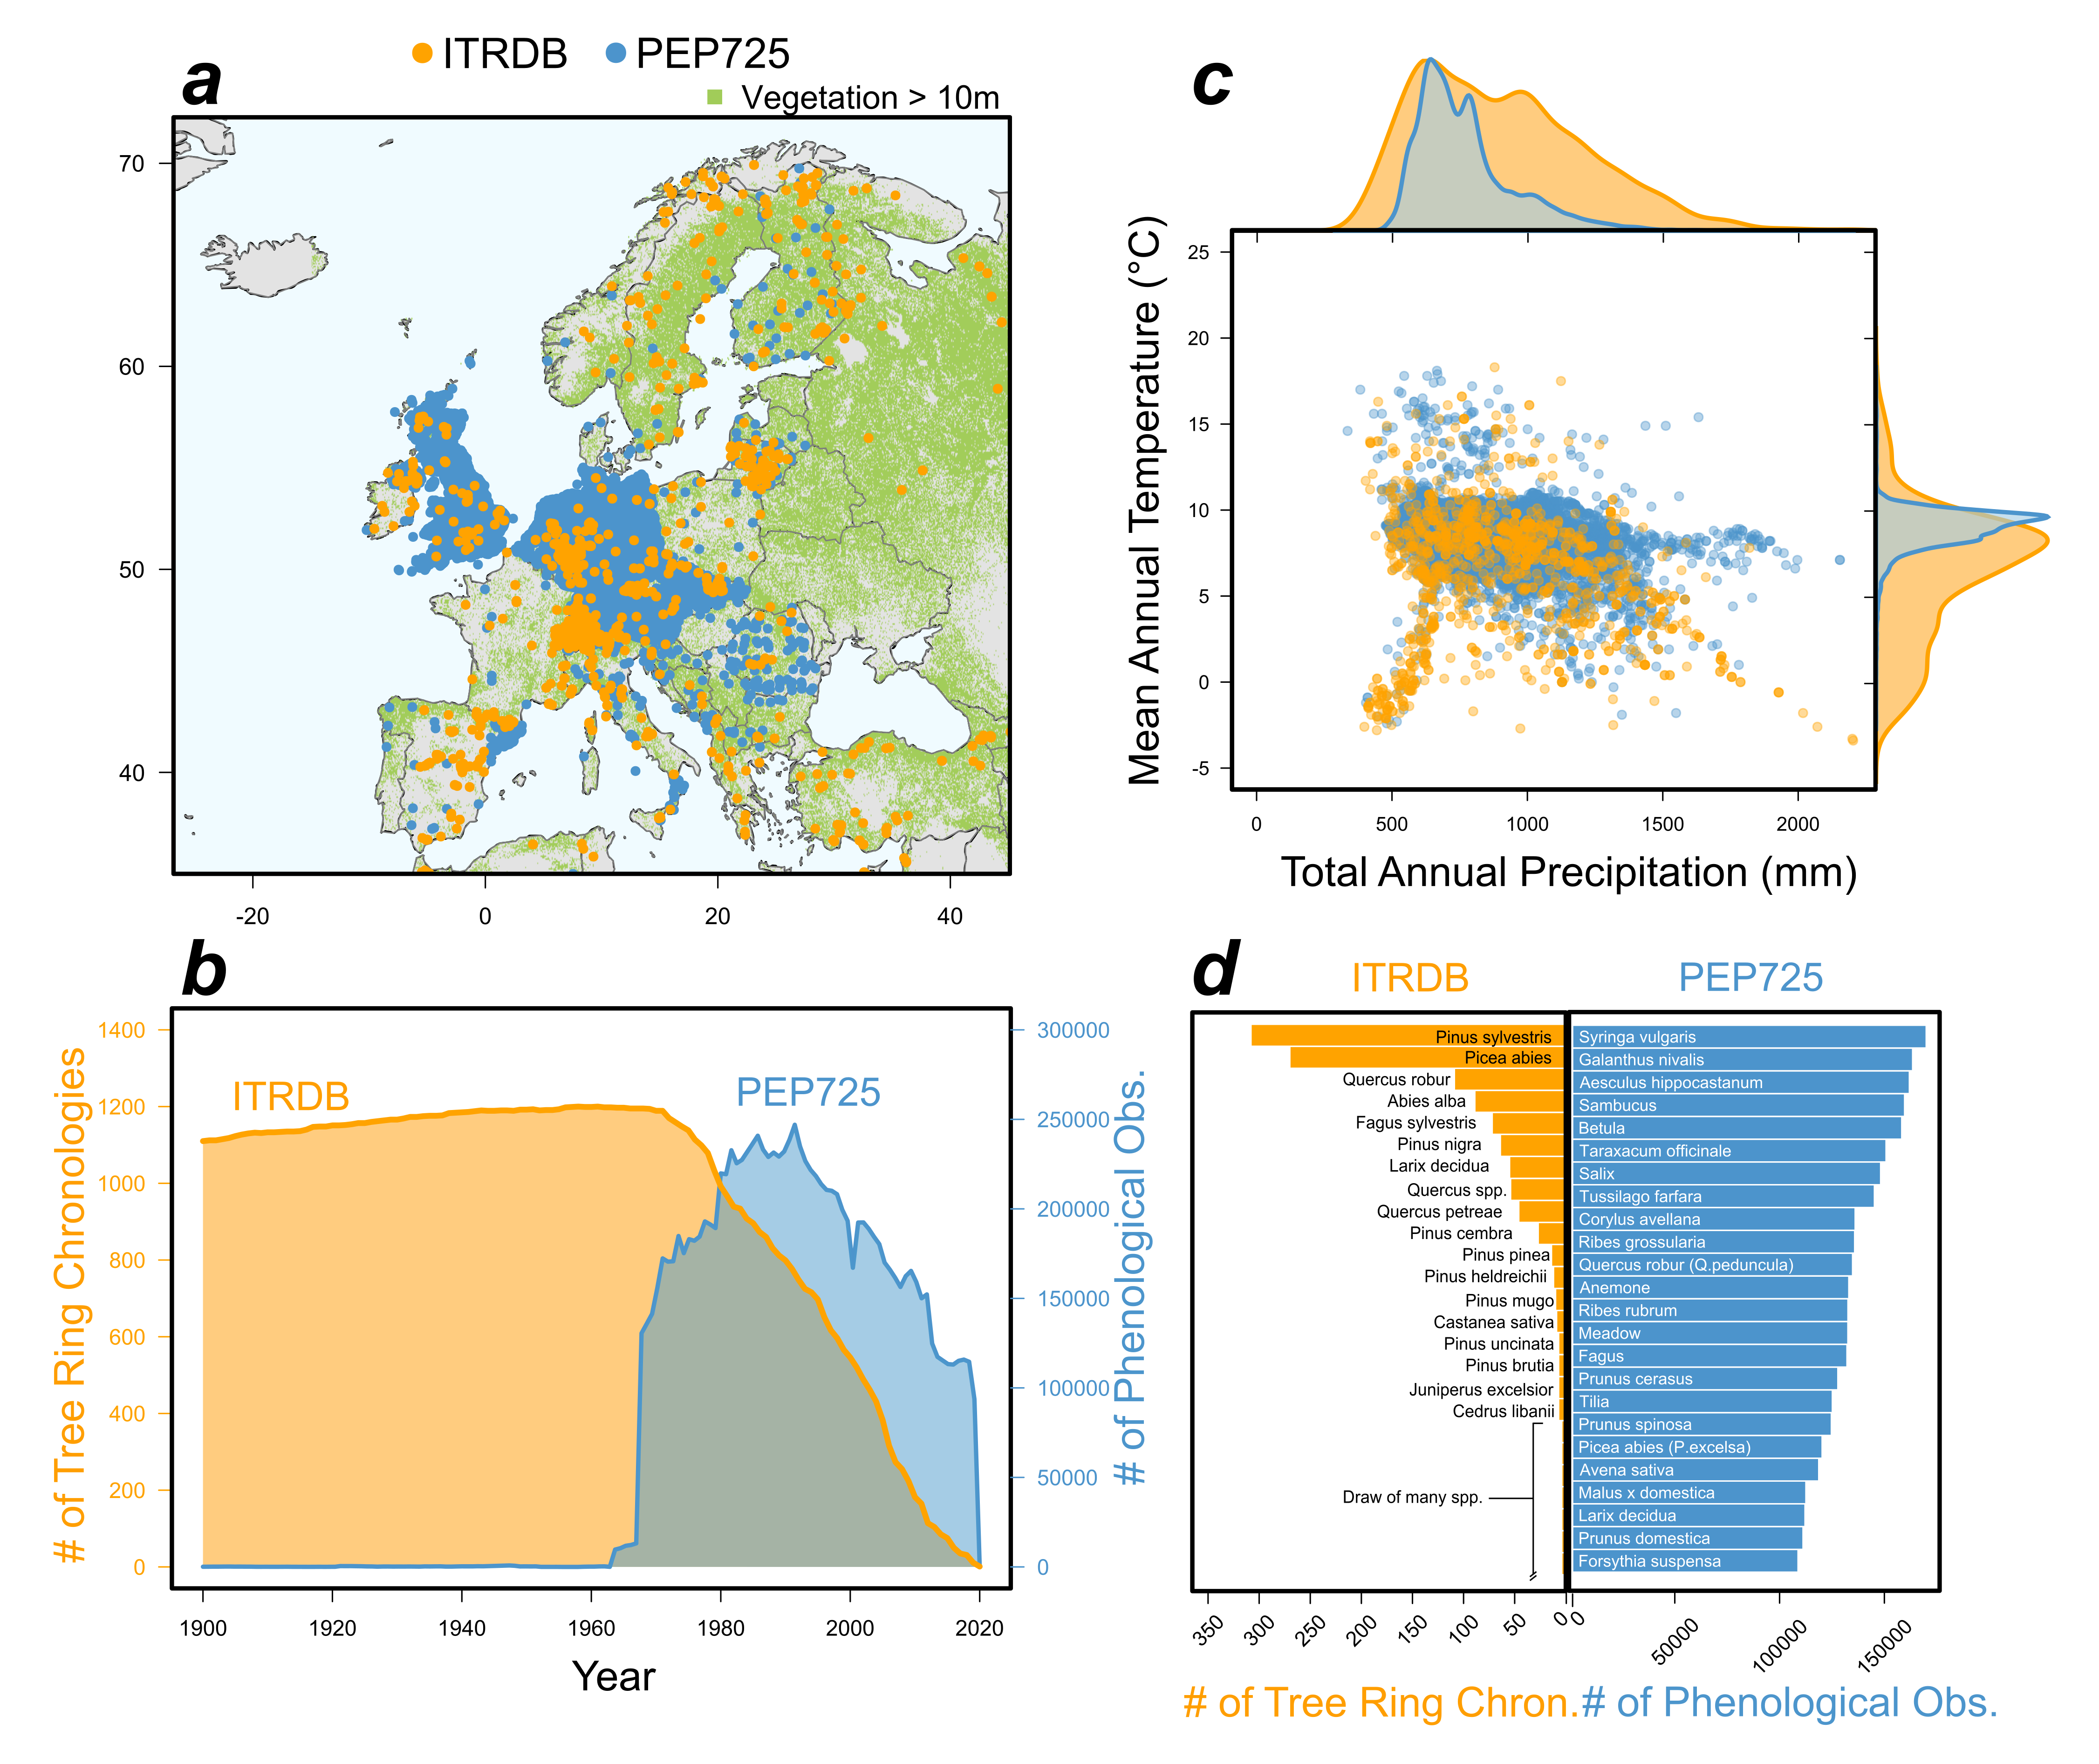
\includegraphics[width=1\textwidth]{..//figures/itrdbpep.png}
\caption{Data overlap between the two major databases of growth (International Tree Ring Data Bank, ITRDB, orange) and plant phenology (Pan European Phenology Project, PEP725, blue). Both databases are compared in terms of their spatial distributions (a), temporal overlaps (b), coverage of environmental conditions in climate space (c) and taxonomical representation (d). Note that the number of tree ring chronologies in (b) are composed by multiple trees per site, typically 10-20. Climatic data from Worldclim database ver. 2.1 at 2.5\degree grid resolution. PEP725 records in d) show the largest records for any given phenophase per species.}
\label{fig:itrbdpep}
\end{figure}

\iffalse
\begin{figure}[h!]
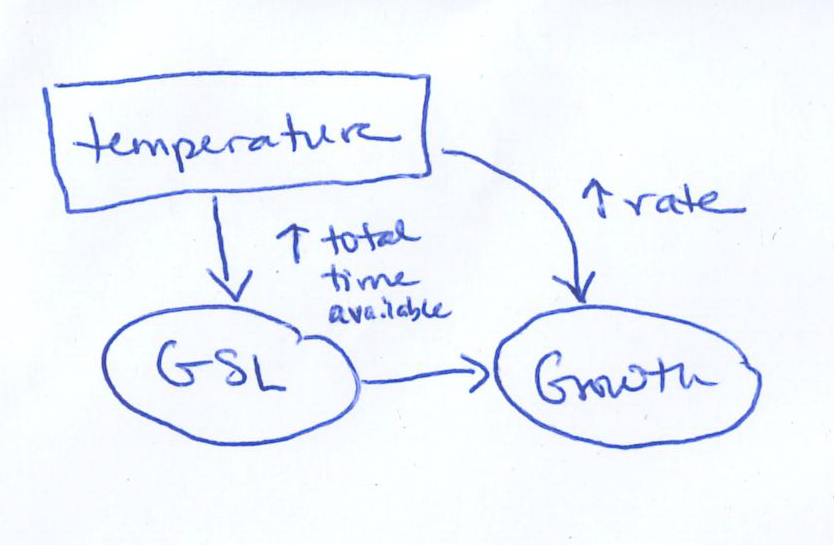
\includegraphics[width=0.5\textwidth]{..//figures/gsltogrowth/gsltogrowth_emw1a.png}
\caption{Idealized simplified version of the world, where resources (including water, N etc.) are abundant and temperatures are never too cool or too hot. In this world, temperature can increase growth directly (through increasing the speed of biological processes, up to some limit) and indirectly, but increasing the absolute available time for those processes to happen and lead to more growth.}
\label{fig:concepbiotime}
\end{figure}


\begin{figure}[h!]
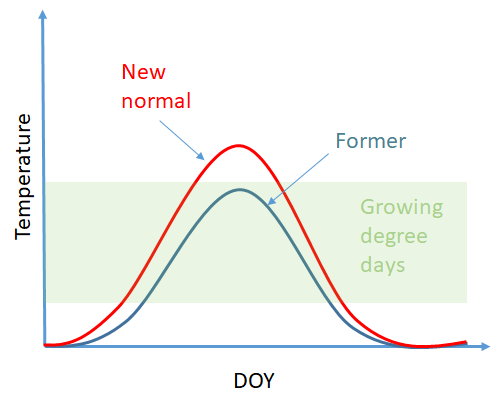
\includegraphics[width=0.75\textwidth]{..//figures/simpletempcurve_fromlucidboard.png}
\caption{Simplified version of how GDD works before and after climate change.}
\label{fig:simpletemp}
\end{figure}
\fi

\clearpage
\section{References}
\bibliography{..//bibtex/grephonbib}
\bibliographystyle{/Users/Lizzie/Documents/git/bibtex/styles/besjournals.bst}





\end{document}


%%%%%%%%%%%%%%%%%%%%%%%%%%%%%%%
%% OLD text -- minus stuff I cut and used already (I think) %%
%%%%%%%%%%% %%%%%%%%%%%%%%%%%%%%

% Text that I cut from the previous draft but may want to REVIEW to see if it's worth fitting in somewhere

Internal/External drivers



 ...though how much longer seasons are depends on what events define the start and end (CITES). 

Perhaps most remarkably unmentioned in the current debate is the prevalence of species-level differences ....

Beyond genetic and developmental constraints, evolutionary history can constrain plant responses\todo{addcites}, though this is effectively unstudied currently as a controller of how growing season length may be limited in affecting growth. Yet most studies testing for such historical effects on plant responses find them... though this is effectively unstudied currently as a controller of how growing season length may be limited in affecting growth. Further, many physiological syntheses find results suggestive of strong phylogenetic relationships, but fail to discuss or test them \citep[e.g., discussions of evergreen versus deciduous phenology without testing for whether this is actually correlated with the deep in time split between gymnosperms and angiosperms,][]{way2010differential}. '

% Previous draft text ... 

\emph{How warmer temperatures increase tree growth, or not}


Elevation and latitude---two major factors that generally shorten seasons, and change a suite of climatic factors---generally lead to less annual growth (new Fig?). Most current work in dendrochronology assumes this relationship and focuses more on how climatic factors shift across these gradients\todo{addcites}. 



\emph{A cross-disciplinary framework for when longer seasons increase tree growth}


\emph{i. External drivers}

\emph{ii. Internal programming}



This focus on climatic signals in tree growth (measured by ring width) is the hallmark of dendrochronology, with the methods in the field generally designed around this aim. Statistical approaches attempt to remove periods of rapid growth with age. Sampling methods, at both the species and individual tree level, 
% Elevation and latitude---two major factors that generally shorten seasons, and change a suite of climatic factors---generally lead to less annual growth (new Fig?) though this relationship in reality may be more messy than many conceptual diagrams suggest. 


Additionally, observational studies must attempt to tease out effects of high temperatures that should accelerate the rate of plant growth, from longer seasons, and from temperatures that are too high and stall growth. Without a solid basis for the underlying temperature response curve, such attempts are likely non-identifiable statistically, and thus could easily report underlying correlations between predictors as signals of different temperature and season-length responses [\colorbox{orange}{More on VPD and/or xylogenesis here?}]. And these complexities must be addressed through a multi-species lens.

Only a handful of studies mentioned species differences, and rarely made predictions based on existing theory. Shifting investment in growth versus reproduction, differences in plant strategies and phylogeny all predict testable variation in how growing season length impacts growth, but have been almost wholly ignored in the current debate. We argue this is because of a lack of cross-disciplinary study. For example, while evolutionary history, ecology and life history theory all predict differences across species, the two major disciplines currently studying this---physiology and dendrochronology---generally study either one species\todo{addcites}, lump all species in a site\todo{addcites}, or divide by one trait \citep[e.g.,][]{dow2022warm}. Research on trends over elevation, which seem foundational to understanding the growth x growing season length relationship, have been on a very limited species list---with almost no comparison across species. % Evolutionary history, ecology and life history theory all predict differences across species, but current analyses generally study either one species\todo{addcites}, or lump all species in a site\todo{addcites}.  

\emph{To the bat-mobile Robin! How to tackle this cross-disciplinary framework}


Dendrochronology provides an invaluable long-term perspective, but using it to understand tree growth beyond climatic factors will require new perspectives and approaches. As rings are easiest to observe in conifers, and conifers often exist in the most extreme climatic places (and thus have more clear signal of climate on growth), dendrochronology has limited data for species where phenology may be most strongly tied to growth---deciduous species, which are mostly angiosperms. Phenology and dendrochronology are somewhat unique fields in biology for their open data that is both geographically and temporally deep; yet the overlap in comparable data due to each field focusing mostly on different suites of species is incredibly limited (\colorbox{orange}{New fig here of PEP725 x ITRB data?}). Further, most standard statistical methods for `standardizing' tree ring data are focused on enhancing climatic signals---which could schmear insights into growing season length or other factors, especially for studies across populations \citep{de2022temperature}. The fundamental model of growth in dendrochronology could use revisiting, especially as new mechanistic understanding from physiology advances. Layering on the complexity of growth depending not only temperature and precipitation, but on vapor pressure deficit, as well as losses in growth that are more episodic (e.g., frost, disease) would help.

% 
ADD Both these [BIOTIC] drivers though can be more episodic and harder to measure, making them more difficult to easily test as mechanisms for limiting growth. In contrast, proxies for competition (such as surrounding tree density and identity), can be more easily measured, but are rarely studied. Mechanistic physiology studies rarely measure (or even include) competition and, given dendrochronology's focus on climatic signal through growth, the field similarly tries to avoid the study or impact of plant competition, even though it is foundational to forest dynamics. And ...  the very established method of merging into average site chronology reduces the chance of seeing competition or biotic factors in play.


Disentangling the effects of major drivers on growth---from growing season length, to temperature, moisture and constraints---likely requires experiments. To date, few experiments have teased out the effects of warmer temperatures versus an longer season, and none---to our knowledge---have carefully measured growth. Such experiments, however, will be critical in establishing a baseline understanding of the role of season length alone in determining growth. And they can compare species robustly. Advancing them to extend the season via early growth or delayed senescence, and layering on heat waves or drought treatments could provide comparable estimates and test lag effects (when sampled multiple years after the manipulations). While these are most easily done for juvenile trees, they could be done on adult trees (given the infrastructure investment), giving the opportunity to measure impacts on reproductive output as well. 
% Comparing the effects of various drivers on growth---from growing season length, to temperature, moisture and constraints---may be impossible from observational or experimental approaches alone. Each is limited ... 


